\documentclass{beamer}
\usepackage{fontspec, siunitx, luacode, xcolor, marvosym, graphicx, verbatim, multicol}
\setbeamertemplate{navigation symbols}{}
\sisetup{output-decimal-marker={,}}

\definecolor{bettergreen}{rgb}{.1,.7,.1}

\usetheme{Luebeck} %dafür muss 2mal kompiliert werden!
\useoutertheme{split} %zugegeben, das verändert nichts, aber alle anderen Optionen sind voll hässlich und wir mögen das Lübeck-Theme =/ Außerdem ist die Beamer Dokumentation auf Spanisch oO
\usecolortheme[named=bettergreen]{structure}
\useinnertheme{rounded}

\title{Raspberry Pi - Webcamsteuerung (Gruppe B)}
\author{Philip Bell, Johannes Visintini}
\date{15. Oktober 2014}

\begin{document}
\begin{frame}[plain]
\titlepage
\end{frame}

\begin{frame} %_________________________________Übersicht_________________________________________
\tableofcontents
\end{frame}

\section{Aufgabenstellung und Werdegang}
\begin{frame}{Aufgabenstellung}
\begin{itemize}
	\item Bau eines Gerüstes inkl. Schwenkvorrichtung für die Kamera
	\item Erstellung eines Webservers mit folgenden Funktionen:
	\begin{itemize}
		\item Anzeige eines Live-Streams
		\item UI zur Steuerung der Kamera
	\end{itemize}
\end{itemize}
\end{frame}

\begin{frame}{Werdegang - Milestones}
\begin{tabular}{l l}
	\textbf{Ende Juni:}			& Raspberry Pi fertig eingerichtet\\
								& Funktionsfähigkeit aller Komponenten getestet\\
	\textbf{Ende August:}			& Befestigung fertiggestellt\\
	\textbf{Mitte September:}		& Webschnittstelle fertiggestellt\\
	\textbf{Ende September:}		& Steuerungssoftware fertiggestellt\\
	\textbf{Anfang Oktober:}	& Präsentation des Praktikums\\
	\textbf{Mitte Oktober:}		& Dokumentation fertiggestellt
\end{tabular}
\end{frame}

\section{Bau des Gerüstes}%_____________________________Konstruktion_______________________________
\begin{frame}{Verkleidung}
\begin{itemize}
	\item<1-> Haltevorrichtung in T-Form\\ $\Rightarrow$ Standfähigkeit und Wandmontage
	\item<2-> Schwenkvorrichtung zur Ausrichtung in vertikaler und horizontaler Ebene
	\item<3-> Pappkarton für dezenten Look
\end{itemize}
\end{frame}


\section{Webserver} %___________________________webseite___________________________________________
\begin{frame}{Webserver}
\only<3>{\center
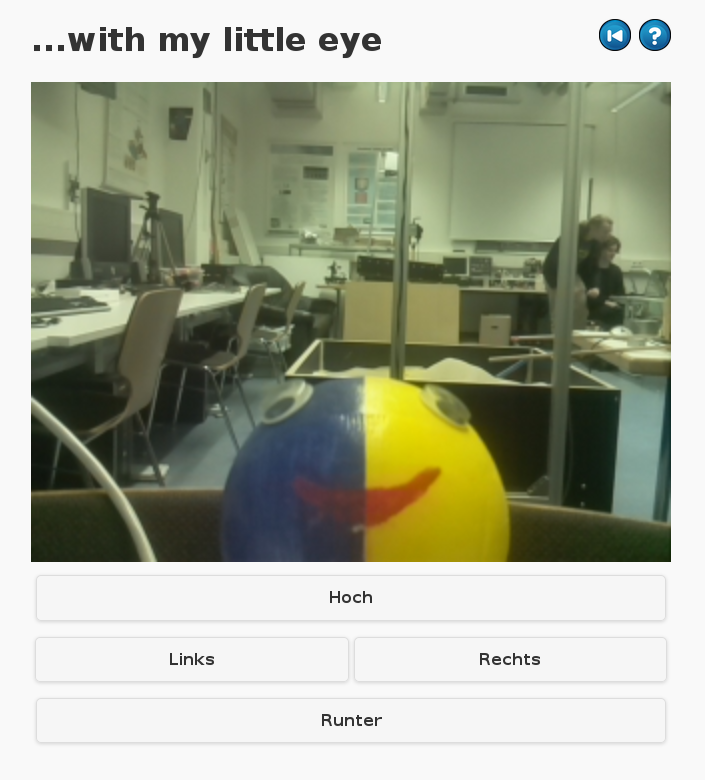
\includegraphics[height=.8\textheight]{websitescreenshot.png}
}
\begin{itemize}
	\item<1-2,4-> Live-Stream, Webseite: mJPG-Streamer
	\item<2,4-> UI: Javascript, JQuery (mobile)
	\item<4-> Sicherheit: Firehol, apache, ssh
\end{itemize}
\end{frame}


\section{Steuerungssoftware}%__________________Steuerungssoftware___________________________________
\subsection{Kontrollfluss}
\begin{frame}{Kontrollfluss}
	\center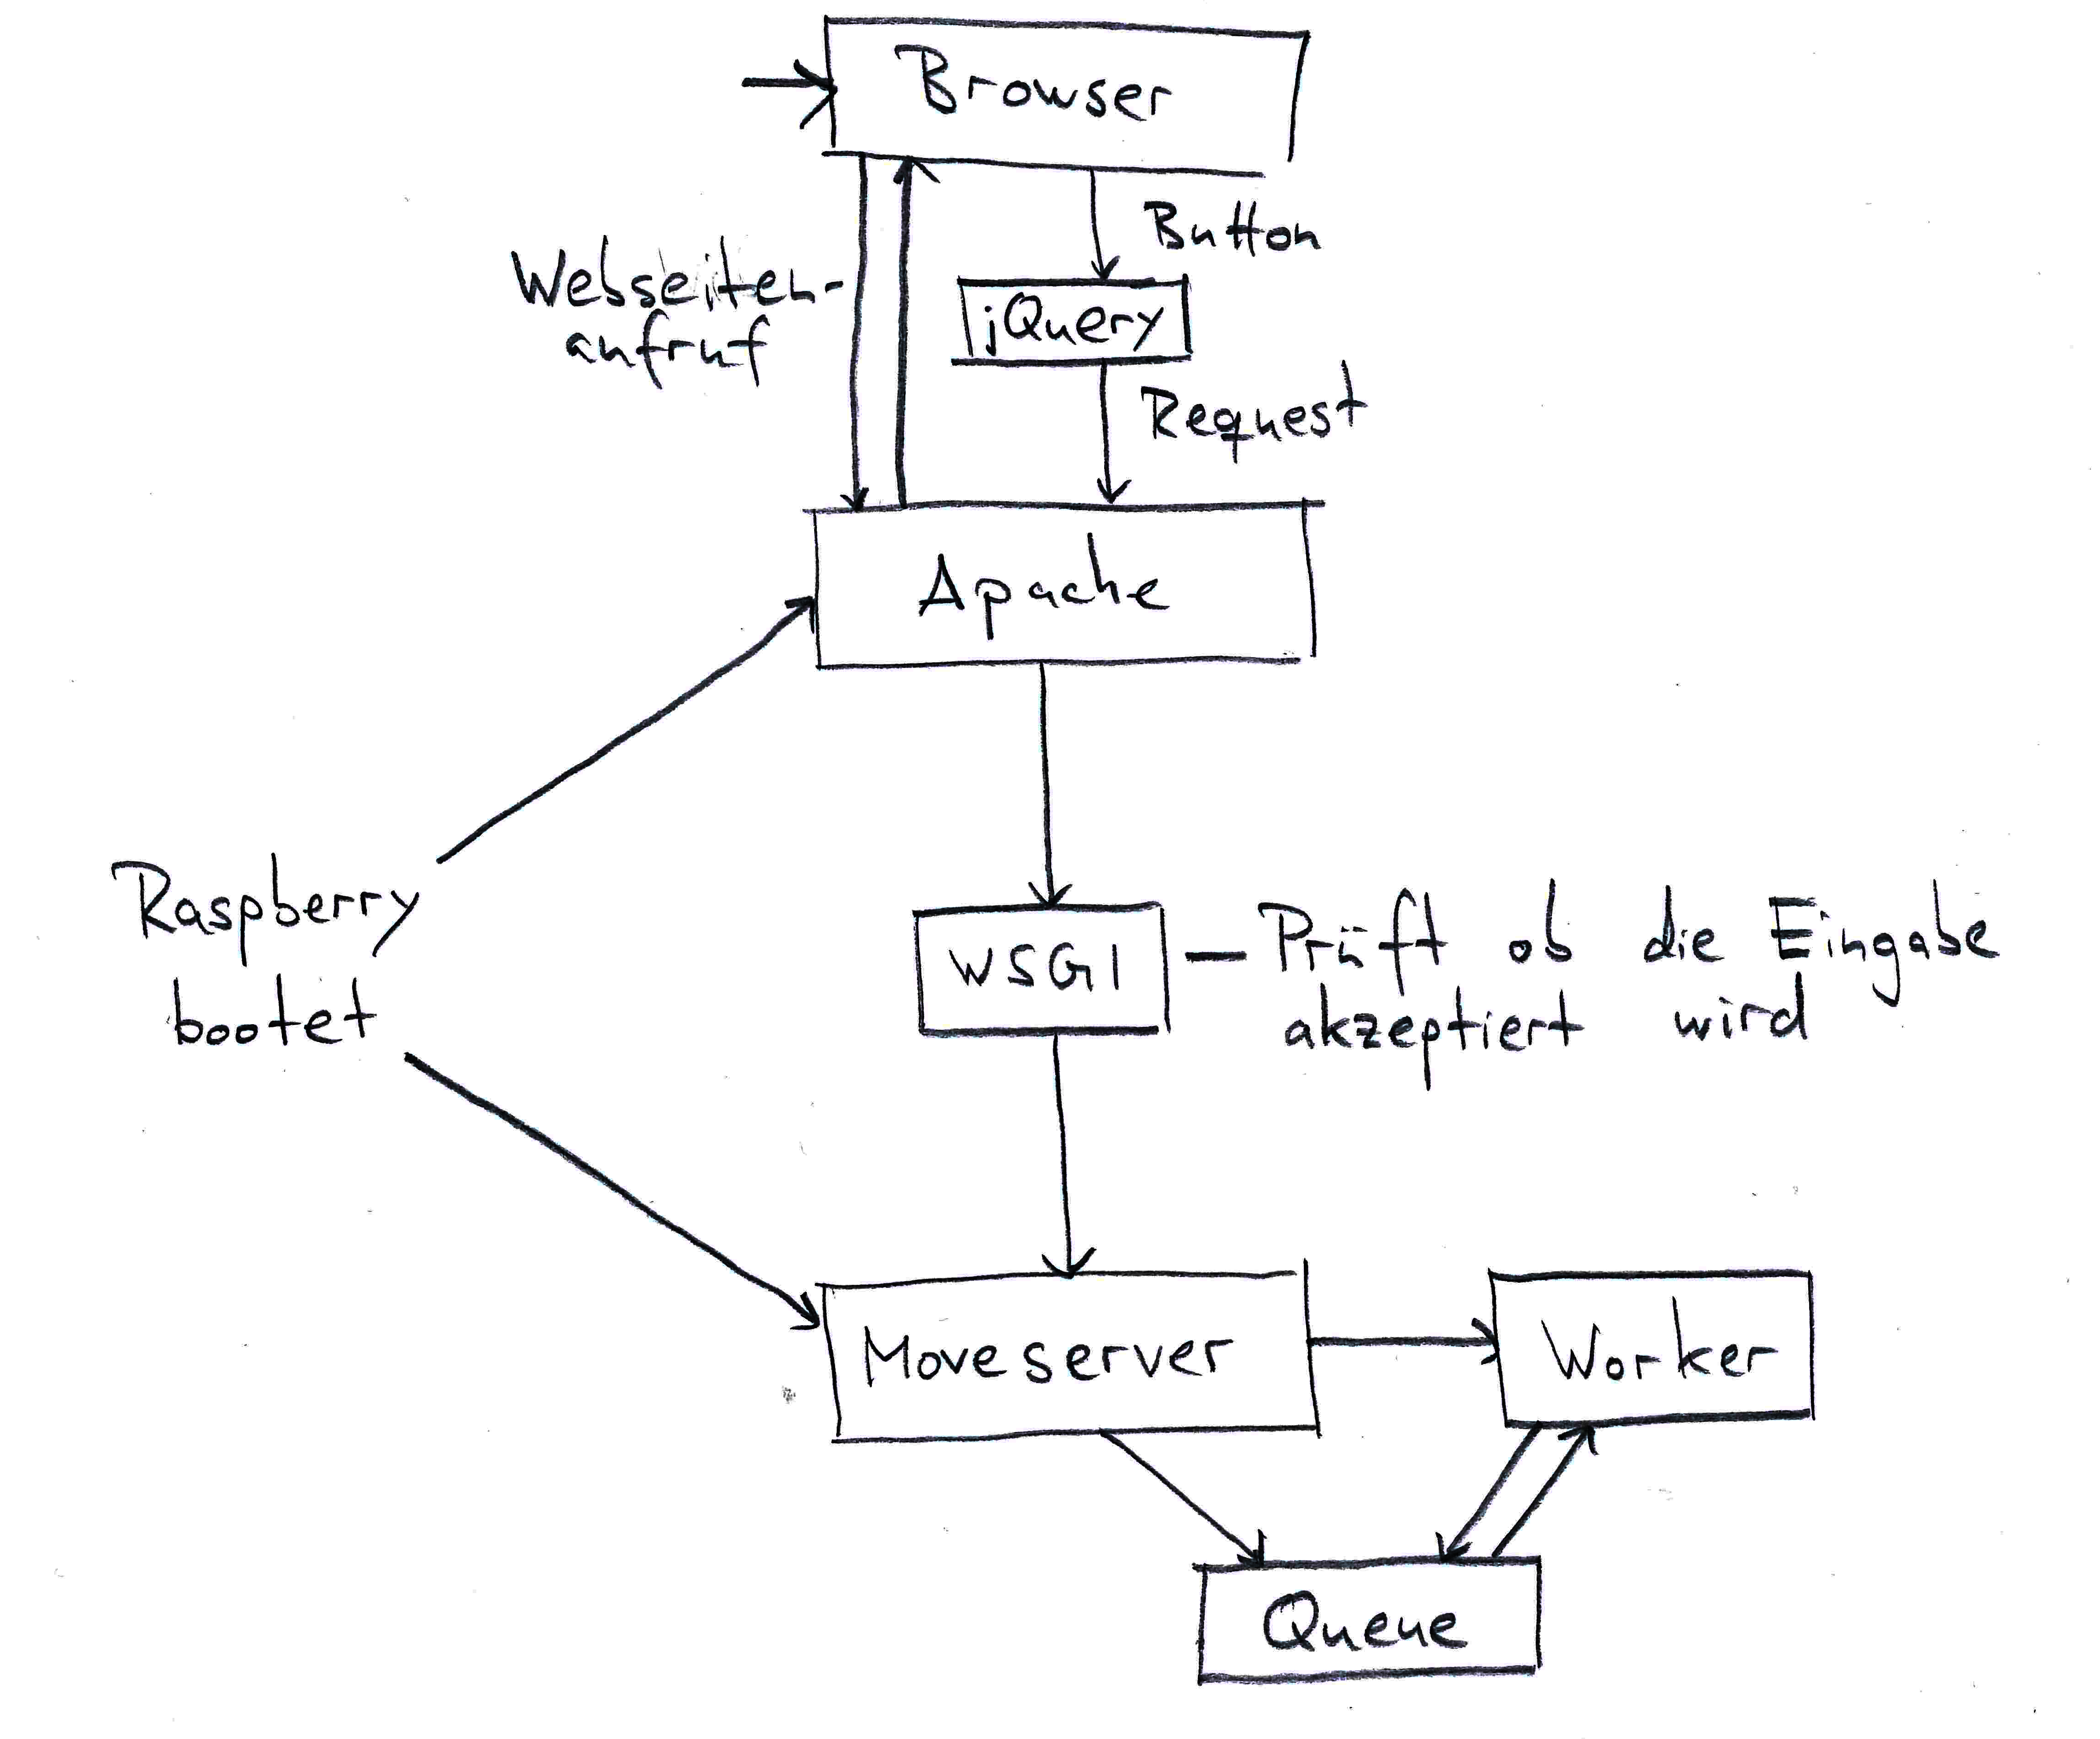
\includegraphics[height=.8\textheight]{kontrollflussdiagramm.png}
\end{frame}

\subsection{moveserver \& move-Funktion}
\begin{frame}{moveserver \& move-Funktion}
	\center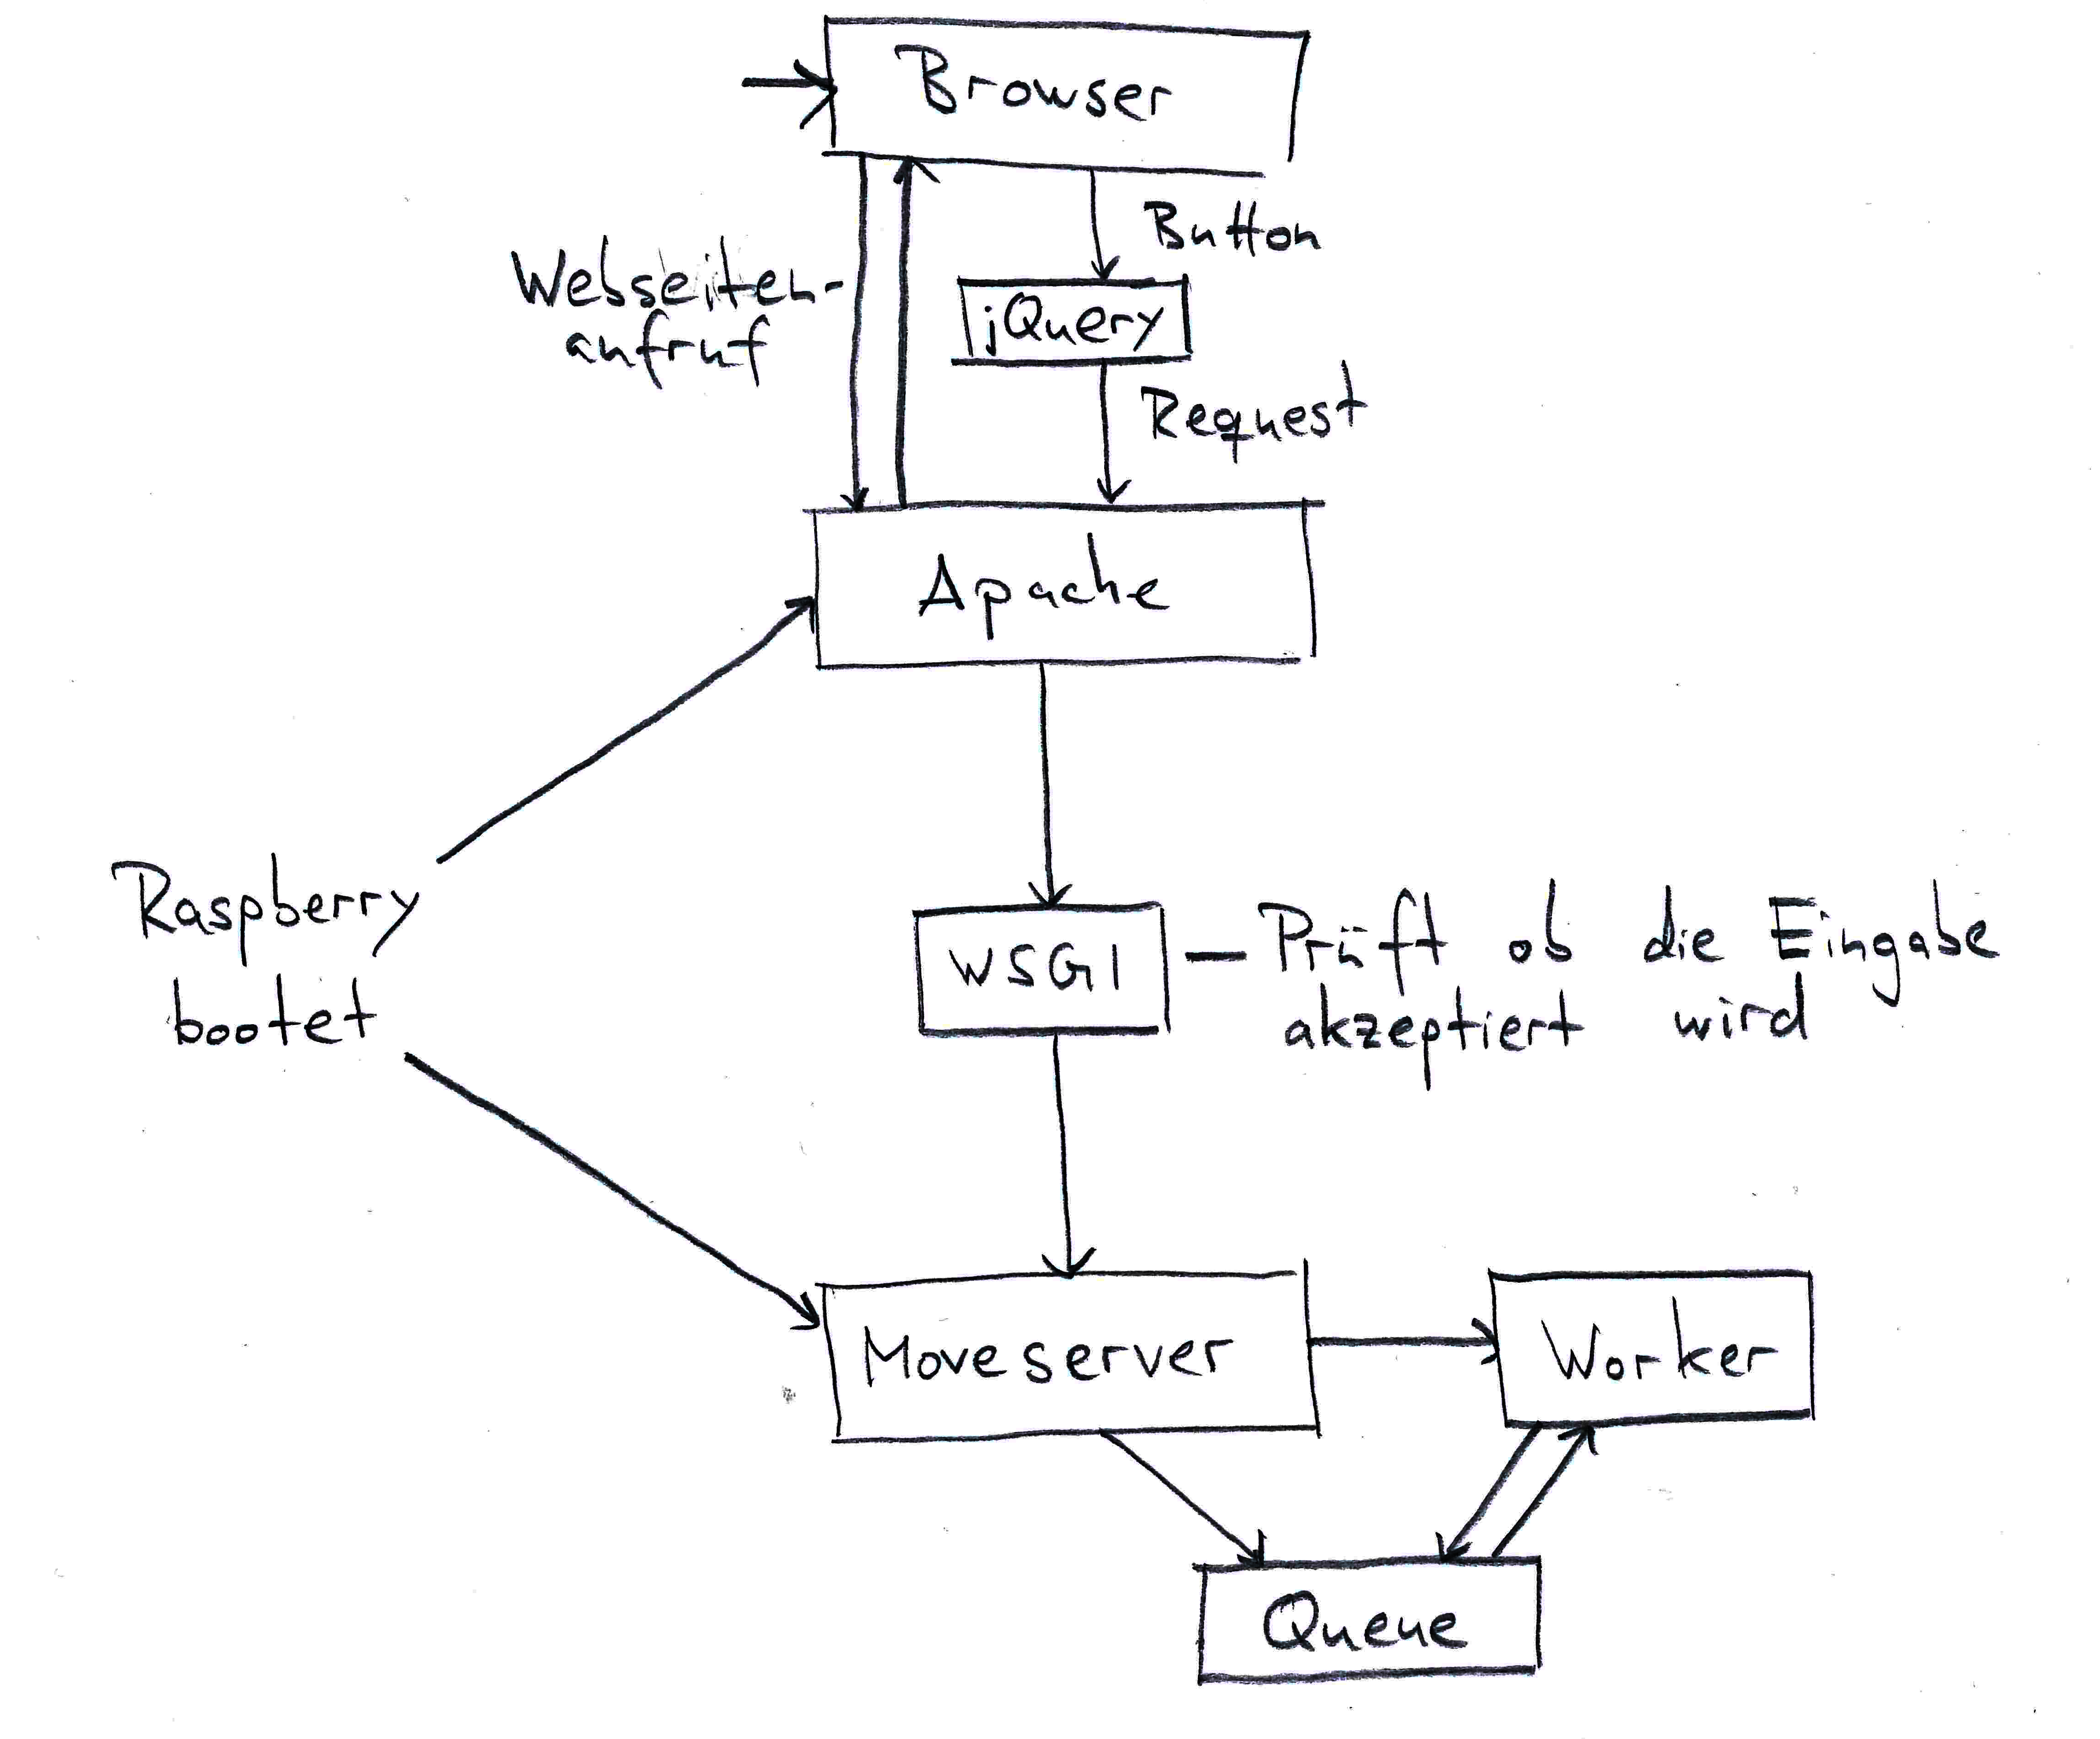
\includegraphics[height=.8\textheight]{kontrollflussdiagramm.png}
\end{frame}


\section{Probleme \& Erweiterungen}%__________________Miscellaneous____________________________________
\subsection{Probleme}
\begin{frame}{Probleme}
\begin{itemize}
	\item<1-> Raspberry Pi defekt, Fehlersuche zeitintensiv\\
		$\Rightarrow$ neuer Raspberry Pi
	\item<2-> Servos brauchen zu viel Strom\\
		$\Rightarrow$ nur in bestimmten Bereichen betreiben (Softwareschranke)\\
		$\Rightarrow$ Verbindungsabbrüche verhindert
	\item<3-> python-Skript für die Servos muss mit root-Rechten laufen\\
		$\Rightarrow$ Service, zur internen Verarbeitung (moveserver)
	\item<4-> Live-Stream hat zu große Latenz\\
		$\Rightarrow$ WLAN-Router überlastet, nicht lösbar
\end{itemize}
\end{frame}


\subsection{Erweiterungen}
\begin{frame}{Erweiterungen (mit Verbesserungsmöglichkeiten)}
\begin{itemize}
	\item<1-> „Standby“
	\item<2-> Neustart bei Netzwerkproblemen
	\item<3-> Prioritätenbehandlung
\end{itemize}
\end{frame}


%_________________Miscellaneous______________________________________
\begin{frame}{Vorführung}
	Vorführung unseres Praktikums ...
\end{frame}	

\begin{frame}{Ende}
	\begin{center}\huge Ende\end{center}
\end{frame}



%Inhaltsverzeichnis:
%Aufgabe
%Bau des Zählwerks
%Algorithmus
% Programm
%Vorführung

%\begin{verbatim}
%\usepackage{siunitx, amsmath}
%\sisetup{output-decimal-marker={,}}
%$\SI{5,32}{\electronvolt}$
%\end{verbatim}

%\begin{frame}[fragile]
%\begin{luacode}
%for k=350,780,5 do
%tex.print("\\color[wave]{",k,"}\\Celtcross Ende ")
%end
%\end{luacode}
%\end{frame}
\end{document}
